% Packages

% Sets

% Formal statements


\begin{document}
\maketitle

\section{Flujo en redes}

El \emph{grafo de Petersen} tiene 10 nodos y 15 aristas y se puede definir a partir
del siguiente dibujo:

\bigskip
\bigskip

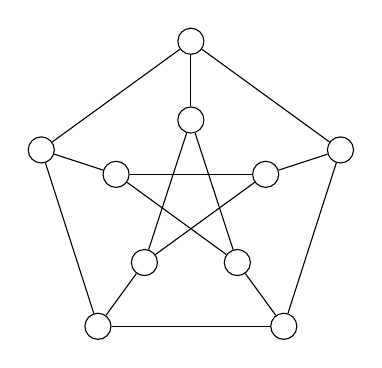
\begin{tikzpicture}
	% Inner nodes
	\node[shape= circle, draw] (N0) at (0.95, 0.31) {};
	\node[shape= circle, draw] (N1) at (0, 1) {};
	\node[shape= circle, draw] (N2) at (-0.95, 0.31) {};
	\node[shape= circle, draw] (N3) at (-0.59, -0.81) {};
	\node[shape= circle, draw] (N4) at (0.59, -0.81) {};
	% Connections between inner nodes
	\draw (N0) -- (N3);
	\draw (N3) -- (N1);
	\draw (N1) -- (N4);
	\draw (N4) -- (N2);
	\draw (N2) -- (N0);
	% Outer nodes
	\node[shape= circle, draw] (N5) at (1.90, 0.62) {};
	\node[shape= circle, draw] (N6) at (0, 2) {};
	\node[shape= circle, draw] (N7) at (-1.90, 0.62) {};
	\node[shape= circle, draw] (N8) at (-1.18, -1.62) {};
	\node[shape= circle, draw] (N9) at (1.18, -1.62) {};
	% Connections between inner nodes and outer nodes
	\draw (N0) -- (N5);
	\draw (N1) -- (N6);
	\draw (N2) -- (N7);
	\draw (N3) -- (N8);
	\draw (N4) -- (N9);
	% Connections between outer nodes
	\draw (N5) -- (N6);
	\draw (N6) -- (N7);
	\draw (N7) -- (N8);
	\draw (N8) -- (N9);
	\draw (N9) -- (N5);
\end{tikzpicture}

\bigskip
\bigskip

En esta sección se le pedirá generar redes de flujo aleatorias cuyas aristas son
versiones dirigidas de las aristas del grafo de Petersen. Si necesita generar
números aleatorios, puede utilizar interfaces como \emph{Random Integer Generator}
de la página \texttt{random.org}. En cada caso se compararán los alogritmos
\texttt{basicFordFulkerson} y \texttt{edmondsKarp} para calcular el flujo máximo
de una red.

\subsection{Algoritmos}
Como parte de la entrega de esta tarea, debe adjuntar un archivo \texttt{.py} o
\texttt{.java} que contenga su implementación tanto de \texttt{basicFordFulkerson}
como de \texttt{edmondsKarp}.

\subsection{Redes muy \emph{nice}}
\begin{enumerate}
	\item Genere dos redes \emph{nice} a partir del grafo de Petersen
		donde las capacidades de las aristas están entre 1 y 50.
	\item De los valores de flujo máximo para cada red. La calificación incluirá
		la verificación de que los algoritmos que usted adjuntó proveen
		ambos ese mismo resultado.
	\item Calcule los costos temporales $\tau_\text{b-F-F}$ y $\tau_\text{E-K}$
		usados por
		cada algoritmo para encontrar el flumo máximo. Debe calcularlos como
		un entero positivo que representa el número de operaciones
		elementales que suceden cuando se ejecuta cada algoritmo con los
		inputs que usted definió. Observe que son cuatro valores en total.

		\textbf{\emph{Alternativa.}} Si no le es posible calcular dichos
		costos temporales de forma exacta, acótelos de la forma
		\[
			L \leq \tau \leq U
		\]
		donde $L, U$ son enteros positivos. En ese caso debe justificar los
		valores de los márgenes de error $\tau - L$ y $U - \tau$.
	\item La pregunta análoga para las complejidades espaciales
		$\sigma_\text{b-F-F}$ y $\sigma_\text{E-K}$. En este caso, la unidad
		de memoria es la \emph{variable} o \emph{apuntador}. En el caso de
		Java por ejemplo, crear la variable \textbf{int} \texttt{number} o
		la variable \texttt{String word} dentro de un algoritmo añade 1 a la
		complejidad espacial.
\end{enumerate}

\subsection{Redes \emph{nice} pero peligrosas}
\begin{enumerate}
	\item Genere dos redes \emph{nice} a partir del grafo de Petersen, tales que
		al menos siete aristas tengan peso entre 1 000 y 10 000, y al menos
		dos aristas tengan peso entre 1 y 5.
	\item Igual que en \textbf{1.2}.
	\item Igual que en \textbf{1.2}.
	\item Igual que en \textbf{1.2}.
\end{enumerate}

\subsection{Redes no-\emph{nice} I}
\begin{enumerate}
	\item Genere tres redes a partir del grafo de Petersen con aristas de
		capacidades entre 10 y 100 tales que
		\begin{enumerate}
			\item Una red no es \emph{nice} porque
				$\delta^+(\sigma) > 0$.
			\item Una red no es \emph{nice} porque $\delta^-(\tau) > 0$.
			\item Una red no es \emph{nice} porque
				$\delta^+(\sigma) > 0$ y $\delta^-(\tau) > 0$.
		\end{enumerate}
	\item Igual que en \textbf{1.2}.
	\item Igual que en \textbf{1.2}.
	\item Igual que en \textbf{1.2}.
\end{enumerate}

\subsection{Redes no-\emph{nice} II}
\begin{enumerate}
	\item Genere dos redes con aristas de capacidades entre 10 y 100 que no son
		\emph{nice} porque tienen dos parejas de aristas antiparalelas.
	\item Igual que en \textbf{1.2}, pero tenga presente que para calcular el
		flujo máximo debe primero convertir cada red en la red \emph{nice}
		equivalente.
	\item Igual que en \textbf{1.2}.
	\item Igual que en \textbf{1.2}.
\end{enumerate}

\subsection{Redes no-\emph{nice} III}
\begin{enumerate}
	\item Genere dos redes con aristas de capacidades entre 1 y 1 000 que no son
		\emph{nice} porque $\delta^+(\sigma) > 0$, $\delta^-(\tau) > 0$ y
		tienen tres parejas de aristas antiparalelas.
	\item Igual que en \textbf{1.5}.
	\item Igual que en \textbf{1.2}.
	\item Igual que en \textbf{1.2}.
\end{enumerate}

%

\section{Distancias mínimas}
\subsection{} Demuestre que Bellman-Ford no es una restricción de Floyd-Warshall de la siguiente manera: Defina dos grafos dirigidos, uno de cuatro nodos y uno de cinco nodos, conexos y CON ciclos negativos, Tales que la fila correspondiente al nodo \emph{source} al final de la ejecución de Floyd-Warshall NO SEA el vector de distancias calculado por Bellman-Ford para ese \emph{source}.

%

\section{Kruskal - \emph{Path Compression}}
En la implementación básica de \texttt{kruskal}, la operación más económica es \texttt{union} con complejidad $O(1)$. Mientras tanto, \texttt{find} es $O(\log n)$. Podemos usar \emph{path compression} para implementar \texttt{smartFind}, que para grafos suficientemente grandes es $O(1)$ y hace que \texttt{kruskal} sea $O(n)$, si ignoramos el paso de ordenar las aristas por peso.

La idea es la siguiente: El llamado \texttt{find(u)} retorna la raíz del árbol al que el nodo \texttt{u} pertenece. Llamemos \texttt{r} a dicho resultado. Suponga que guardamos una referencia \textbf{int} \texttt{temp= r}. En el camino desde \texttt{u} hasta \texttt{r}, probablemente visitamos los nodos $\mathtt{v_1, v_2,..., v_t}$. Usando la referencia \texttt{temp}, volvemos a visitar estos nodos, esta vez haciendo que apunten directamente a \texttt{r}.

\subsection{} Implemente \texttt{smartFind} y úselo para reemplazar \texttt{find} en la versión básica de \texttt{kruskal}.

\subsection{} Ahora a medida que se ejecuta el algoritmo, el arreglo \texttt{heights} deja de almacenar las alturas de los árboles que representan los conjuntos de la partición. ¿Por qué esto no afecta el tiempo de ejecución de \texttt{union}?

\subsection{} Explique qué sucede si se implementa \texttt{kruskal} con \texttt{badUnion} y \texttt{smartFind}. Determine el orden de complejidad analizando el peor de los casos. No hace falta una demostración formal.

%

\section{Algoritmo de Jarnik-Prim.}
Este es otro algoritmo avaro que calcula un mínimo árbol de recubrimiento. Suponga que los nodos de $G$ son $\{0,1,2,...,n-1\}$ y que $G$ es conexo.

\begin{itemize}
\item[] 
\item El conjunto $B$ consiste de nodos y se inicializa con $B \leftarrow \{0\}$; El conjunto $T$ consiste de aristas y se inicializa con $T \leftarrow \emptyset$.
\item[] 
\item El conjunto $A$ de aristas se ordena por pesos.
\item[] 
\item \texttt{<loop>} Se busca en $A$ el eje más liviano $\mathbf{e} = \{u,v\}$ tal que $u \in B \ \land \ v \notin B$. Entonces se hace la actualización $B \leftarrow B \cup \{u,v\}$; $T \leftarrow T \cup \{\mathbf{e}\}$. Se detiene cuando $\# B = n$.
\item[] 
\item Retorna $T$.
\item[] 
\end{itemize}

\subsection{} Implemente el algoritmo y llámelo \texttt{jPrim}. Asegúrese de que termine exitosamente aún cuando $G$ no es conexo. Compare esto con el resultado de \texttt{kruskal} para grafos no conexos.
\subsection{} La inicialización por defecto es $B \leftarrow \{0\}$; $T \leftarrow \emptyset$. Sea \texttt{jPrim1} el algoritmo que resulta de reemplazar la inicialización por $B \leftarrow \emptyset$; $T \leftarrow \{\mathbf{e}\}$, donde \textbf{e} es la arista más corta. ¿Es diferente el resultado? explique su respuesta.
%
\end{document}
